To fulfil  the purpose of prototype and reduce the cost of implementation we implemented two fully featured drawers that includes weight sensing and visual output and four basic drawers that consists of only visual output modules.
The fully featured drawer contain one load cell(Model), the load cell is employed to measure the pressure of equipments that is generally stored in the drawers. The signal of the load cell is then amplified via an amplifier to feed into the Arduino. Moreover, The visual feed back module is made of three LEDs that are operated by the Arduino. Similarly, the basic drawers work based on same principle; however the there is no weight sensing technique. The schematic  \ref{fig:example_circuit}  shows the hardware implementation of the full featured drawer. Also the figure  \ref{fig:example_drawer} shows the visual demonstration of drawer. The transparent plate attached with the load cell is used to place equipment to over it to measure the wight. The load cell below measure the pressure due to the placement of equipment over the visible board. 
%
\begin{figure}
	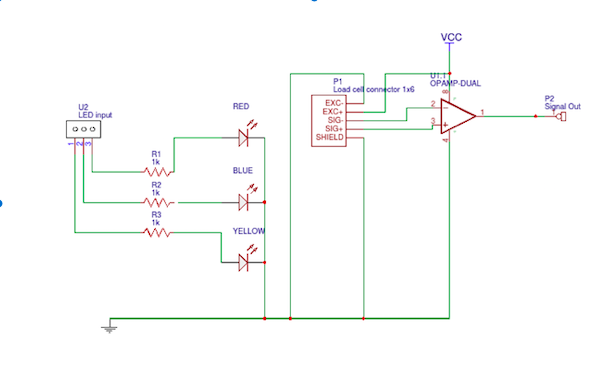
\includegraphics[width=1\columnwidth]{figures/drawer_circuit}
	\caption{Circuit diagram of smart drawer}~\label{fig:example_circuit}
\end{figure}
\begin{figure}
	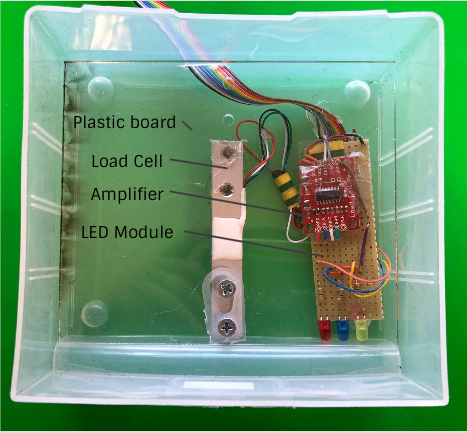
\includegraphics[width=1\columnwidth]{figures/drawer.png}
	\caption{Hardware configuration of a smart drawer}~\label{fig:example_drawer}
\end{figure}
%
\\